% Theorie Einführung
\section{Theoretischer Hintergrund}
\label{sec:theorie}
Man kann hier wunderbar Zitate einpflegen (\citealp{Statista2018}) oder auch (\cite{Statista2018}) oder auch (\citeauthor{Statista2018}).

\begin{wrapfigure}[10]{r}{0.5\textwidth}
    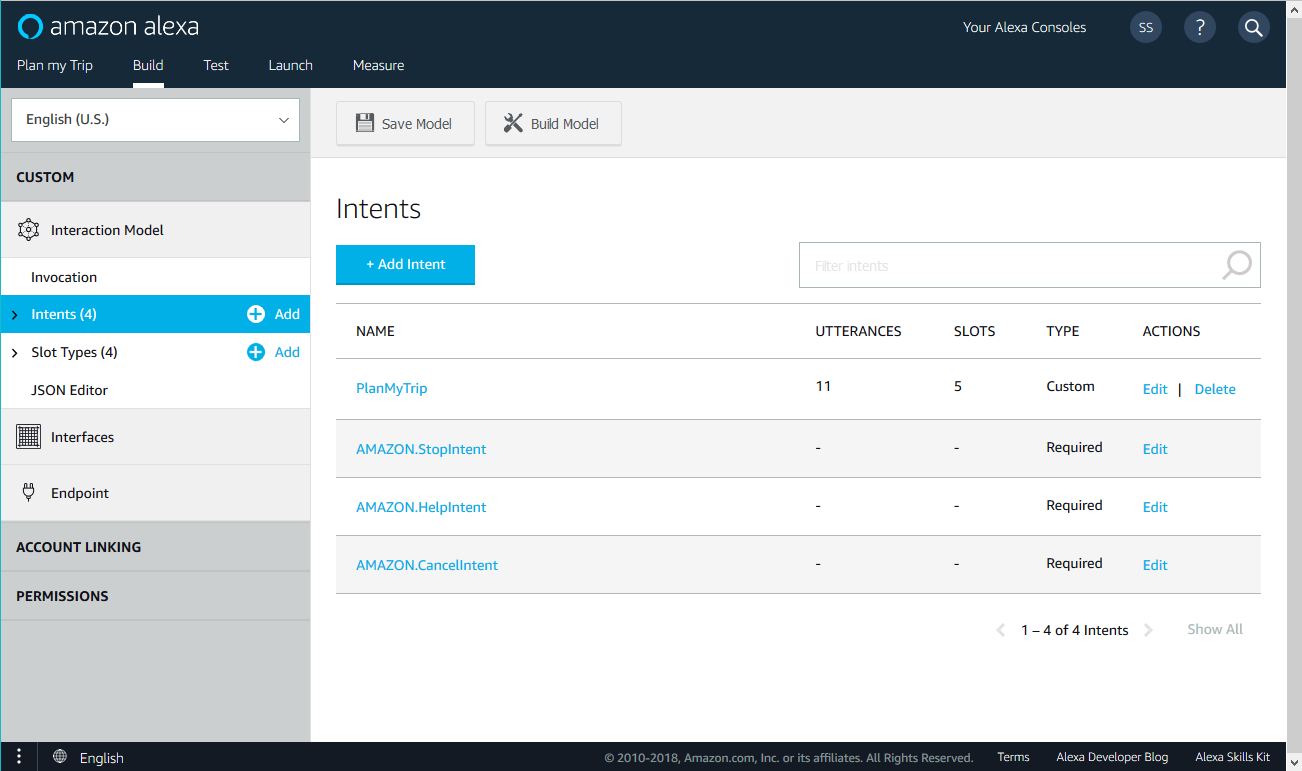
\includegraphics[width=0.48\textwidth]{resources/images/amazon_dev_console.png}
    \caption{Demobild}
    \label{fig:demobild2}
\end{wrapfigure}

Man kann auch Bilder im Text einbinden: Dafür muss man lediglich eine wrapfigure erstellen, die entsprechende Grafik beinhaltet. Durch die Paramter kann man das Verhalten der Wrapfigure beeinflussen um so beispielsweise die Breite anzupassen.

Zudem gibt es die Möglichkeit, auf einfache Weise Bilder über die gesamte Breite einzufügen:
\begin{figure} [ht]
        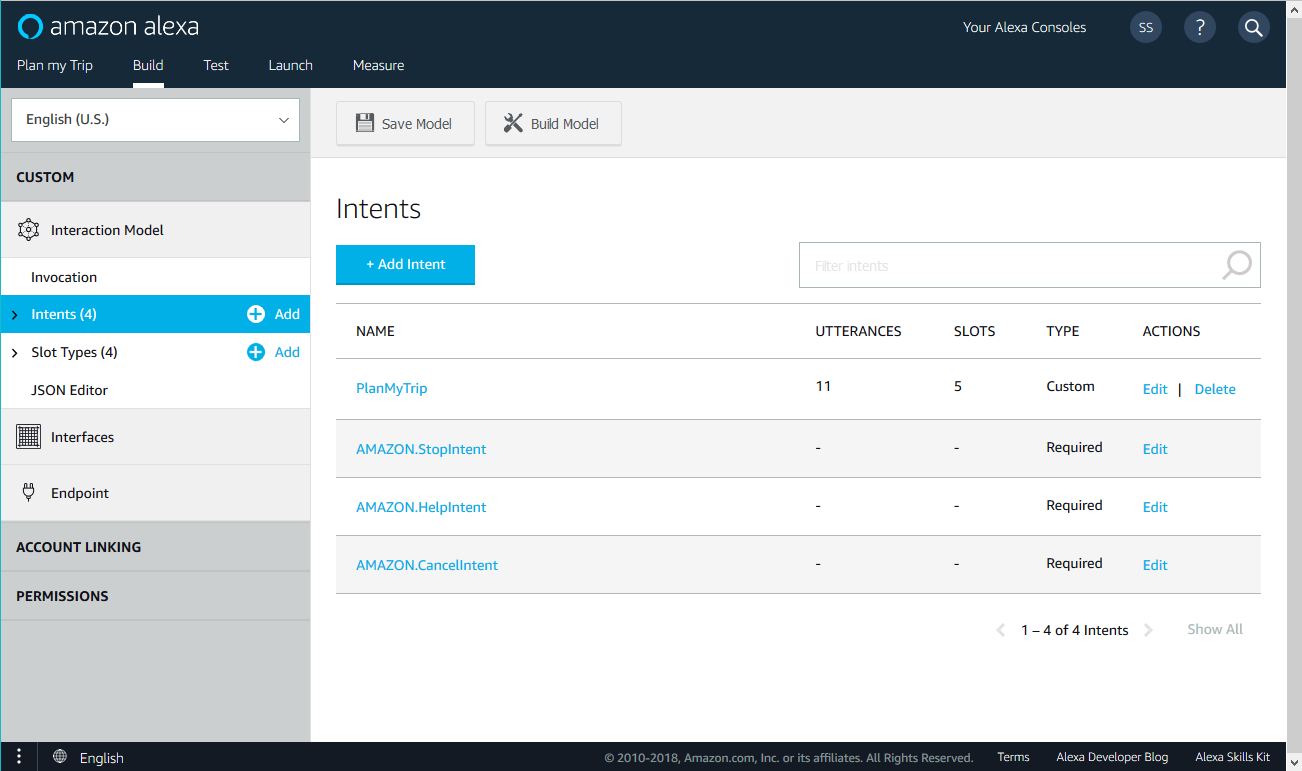
\includegraphics[width=\textwidth]{resources/images/amazon_dev_console.png}
        \caption{Demobild}
        \label{fig:demobild}
\end{figure}

Auf die Abbildung \ref{fig:demobild} kann man innerhalb des Textes referenzieren.